\que{Н-преобразования отсчетной конфигурации. 
Понятие об H-индифферентных и Н-инвариантных тензорах, примеры.}

\paragraph{H-преобразования отсчетной конфигурации.} Определяющие соотношения соответствуют движению сплошной среды из $\mathring{\mathcal{K}}$ в $\mathcal{K}$. Если мы в качестве отсчетной конфигурации выберем другую отсчетую конфигурацию $\overset{\ast}{\mathcal{K}}$, то движению среды $\overset{\ast}{\mathcal{K}} \to \mathcal{K}$ будут соответствовать, вообще говоря, некоторые другие определяющие соотношения, которые можно записать в виде
\begin{equation*}
	\overset{\ast}{\Lambda} = \overset{\cup}{f^{\ast}}(\overset{\ast}{\mathcal{R}}),
\end{equation*} 
где $\overset{\ast}{\Lambda}$ и $\overset{\ast}{\mathcal{R}}$ --- какие-либо активные и реактивные переменные, соответствующие движению $\overset{\ast}{\mathcal{K}} \to \mathcal{K}$. Оператор $\overset{\cup}{f^{\ast}}$, вообще говоря, может отличаться от $\overset{\,\cup}{f}$ (т.е. от того что в Вопросе 29, из аксиомы принципа термодинамически согласованного детерминизма). Основная задача заключается в том, чтобы найти такие отсчетные конфигурации $\overset{\ast}{\mathcal{K}}$, что движение $\overset{\ast}{\mathcal{K}} \to \mathcal{K}$ не изменяет оператора $\overset{\,\cup}{f}$, т.е. имеет место соотношение
\begin{equation*}
	\overset{\ast}{\Lambda} = \overset{\,\cup}{f}(\overset{\ast}{\mathcal{R}}).
\end{equation*}
Найдем эти конфигурации $\overset{\ast}{\mathcal{K}}$.

Положение одной и той же точки $\mathcal{M}$ в $\mathring{\mathcal{K}}$ или в $\overset{\ast}{\mathcal{K}}$ характеризуют радиус-векторы $\mathring{\mathbf{x}}$ или $\overset{\ast}{\mathbf{x}}$ соответсвенно
\begin{equation*}
	\mathring{\mathbf{x}} = \mathring{\mathbf{x}}(X^i), \quad 
	\overset{\ast}{\mathbf{x}} = \overset{\ast}{\mathbf{x}}(X^i),
\end{equation*}
причем $\mathring{\mathbf{x}}$ и $\overset{\ast}{\mathbf{x}}$ связаны дифференцируемым преобразованием:
\begin{equation*}
	\mathring{\mathbf{x}} = \mathring{\mathbf{x}}(\overset{\ast}{x}^i). 
\end{equation*}

\begin{figure}[H]
	\centering
	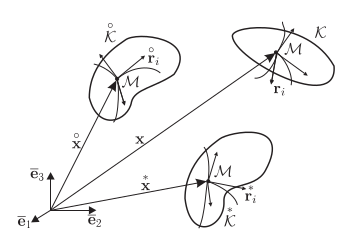
\includegraphics[width=0.6\linewidth]{img/que31}
	\caption{Положение точки $\mathcal{M}$ в актуальной и различных отсчетных конфигурациях}
	\label{fig:que31}
\end{figure}

Для одной и той же точки $\mathcal{M}$ можем ввести локальные базисы и метрические матрицы в $\mathring{\mathcal{K}}$ и аналогично  $\overset{\ast}{\mathcal{K}}$ (ну это вроде не надо расписывать, понятно как), а также градиенты деформации при преобразованиях $\mathring{\mathcal{K}} \to \mathcal{K}$, $\overset{\ast}{\mathcal{K}} \to \mathcal{K}$ и $\mathring{\mathcal{K}} \to \overset{\ast}{\mathcal{K}}$ соответственно:
\begin{equation*}
	\mathbf{F} = \mathbf{r}_i \otimes \mathring{\mathbf{r}}^i, \quad \overset{\ast}{\mathbf{F}} = \mathbf{r}_i \otimes \overset{\ast}{\mathbf{r}}^i, \quad \mathbf{H} = \overset{\ast}{\mathbf{r}}_i \otimes \mathring{\mathbf{r}}^i.
\end{equation*}

Тензор $\mathbf{H}$, описывающий движение из $\mathring{\mathcal{K}}$ в $\overset{\ast}{\mathcal{K}}$, связывает градиенты деформации $\mathbf{F}$ и $\overset{\ast}{\mathbf{F}}$: 
\begin{equation*}
	\mathbf{F} = \overset{\ast}{\mathbf{F}} \cdot \mathbf{H}, \quad \overset{\ast}{\mathbf{F}} \cdot \mathbf{H}^{-1}.
\end{equation*}

(в целом можно было бы этой фразой только ограничется, но для контекста надо было как будто)

\paragraph{$H$-индифферентные и $H$-инвариантные тензоры.} 
\begin{definition*}
	Тензор $\Omega$ называют $H$-\textit{индифферентным}, если его компоненты не изменяются при переходе из одной отсчетной конфигурации $\overset{\ast}{\mathcal{K}}$ в другую $\mathring{\mathcal{K}}$:
	\begin{equation*}
		\mathring{\Omega}^{i_1, \dotsc, i_n}(\mathring{\mathbf{x}}) = \overset{\ast}{\Omega}^{i_1, \dotsc, i_n}(\overset{\ast}{\mathbf{x}}).
	\end{equation*}
\end{definition*}

\begin{definition*}
	Тензор $\Omega$ называют $H$-\textit{инвариантным}, если он не изменяется при переходе из $\mathring{\mathcal{K}}$ в $\overset{\ast}{\mathcal{K}}$, т.е.
	\begin{equation*}
		\mathring{\Omega}(\mathring{\mathbf{x}}) = \overset{\ast}{\Omega}(\overset{\ast}{\mathbf{x}}).
	\end{equation*}
\end{definition*}


\paragraph{Примеры. } Метрический тензор $\mathbf{E}$ одинаков во всех конфигурация, т.е. он является $H$-инвариантным, в чем можно убедиться и непосредственной проверкой. 
\begin{equation*}
	\overset{\ast}{\mathbf{E}} = \overset{\ast}{\mathbf{r}}_i \otimes \overset{\ast}{\mathbf{r}}^i = \mathbf{H} \cdot \mathring{\mathbf{r}}_i \otimes \mathring{\mathbf{r}}^i \cdot \mathbf{H}^{-1} = \mathbf{H} \cdot \mathbf{E} \cdot \mathbf{H}^{-1} = \mathbf{H} \cdot \mathbf{H}^{-1} = \mathbf{E}.
\end{equation*}

Градиент деформации $\mathbf{F}$ не является ни $H$-инвариантным, ни $H$-индифферентным, т.к. он преобразуется по другим законам. Также и $\overset{(n)}{\mathbf{C}}$, $\overset{(n)}{\mathbf{A}}$, $\overset{(n)}{\mathbf{G}}$ и $\overset{(n)}{\mathbf{g}}$. Как они преобразуются можно посмотреть на 195 стр. Димитриенки. 

Только правая мера Альманзи $\mathbf{G}^{-1}$, а значит и $\overset{I}{\mathbf{G}}$, являются $H$-индифферентными. Также стр. 195.

Тензор Коши $\mathbf{T}$ $H$-инвариантен, чего нельзя сказать о других тензорах напряжений.
